\documentclass[dcc]{fcfmcourse}
\usepackage{teoria}
\usepackage[utf8x]{inputenc}
\usepackage{amsmath}
\usepackage{amsfonts,setspace}
\usepackage{listings}
\usepackage{color}
\usepackage{xcolor}
\usepackage{listings}
\lstset{basicstyle=\ttfamily,
  showstringspaces=false,
 % commentstyle=\color{red},
  %keywordstyle=\color{blue}
}
\usepackage{cancel}
\usepackage{hyperref}
\usepackage{epstopdf}
\usepackage{fancyhdr}
\pagestyle{fancy}
%\cfoot{``In mathematics the art of asking questions is more valuable than solving problems" \\ Georg Cantor}
\definecolor{pblue}{rgb}{0.13,0.13,1}
\definecolor{pgreen}{rgb}{0,0.5,0}
\definecolor{porange}{rgb}{0.9,0.5,0}
\definecolor{pgrey}{rgb}{0.46,0.45,0.48}

\lstset{language=Java,
  showspaces=false,
  showtabs=false,
  breaklines=true,
  showstringspaces=false,
  breakatwhitespace=true,
  commentstyle=\color{porange},
 % keywordstyle=\color{pblue},
  stringstyle=\color{pgreen},
  basicstyle=\ttfamily,
  moredelim=[il][\textcolor{pgrey}]{$ $},
  moredelim=[is][\textcolor{pgrey}]{\%\%}{\%\%}
}
\renewcommand{\figurename}{Figura}

\newenvironment{codebox} {\small \ttfamily \obeylines \begingroup \setstretch{-2.4}} {\endgroup}

\title{Tarea 2}
\course[CC3102]{Teoría de la Computación}
\professor{Gonzalo Navarro}
\assistant{Manuel Cáceres}
\assistant{Ian Letter}

% Si pasas el comando usedate a la clase, la fecha aparecerá bajo la lista de auxiliares.
% Puedes usar el formato de fecha por defecto de latex (y traducirla usando babel)
% o puedes escribir lo que quieras con el comando \date.
% \date{1 de Septiembre, 2015}

\begin{document}
\maketitle
\begin{center}
Fecha de entrega : 2 de Diciembre del 2016
\end{center}
\vspace{-1ex}

\section*{Descripción}
Considere un conjunto de colores \textbf{$\mathcal{K} = \{Azul, Rojo, Verde, Blanco, Negro\}$}. Un \textit{tablero} es una grilla $\mathcal{T}:\{1,\ldots,50\} \times \{1,\ldots,50\} \mapsto \mathcal{K}$, donde $\mathcal{T}[i,j]=k$ se interpreta como ``$\mathcal{T}$ está coloreado con el color $k$ en la casilla ubicada en el $i$-ésima fila (de abajo hacia arriba) y $j$-ésima columna (de izquierda a derecha)''.\\

Una \textit{pluma} $\mathcal{P}(posx,posy,col,mod,dir)$ es un objeto que puede moverse por un tablero y cambiar los colores de sus casillas. La pluma tiene un color propio y puede estar alzada o en contacto con el tablero. Si la pluma se mueve estando en contacto con el tablero, las casillas que visita cambian su color al color de la pluma. Formalmente, una pluma $\mathcal{P}$ está determinada por los valores $posx,posy,col,mod,dir$.
\begin{itemize}
\item Si $\mathcal{P}.posx = i$, $\mathcal{P}.posy=j$, la pluma se encuentra en la posición $\mathcal{T}[i,j]$ del tablero.
\item Si $\mathcal{P}.col = k \in \mathcal{K}$, el color de la pluma es $k$.
\item El valor $\mathcal{P}.mod \in \{arriba, abajo\}$ indica si la pluma está en contacto con el tablero y puede cambiar el color de las casillas al moverse ($\mathcal{P}.mod=abajo$), o si se encuentra alzada y puede moverse sin cambiar el color del tablero ($\mathcal{P}.mod=arriba$).
\item Finalmente, $\mathcal{P}.dir \in \{S,N,E,O\}$ representa la dirección en la que puede avanzar la pluma (sur, norte, este, oeste).
\end{itemize}

El objetivo de esta tarea es implementar un intérprete para una gramática libre  del contexto que permita escribir patrones complejos de movimiento y coloramiento de una pluma sobre un tablero. Su programa iniciará un tablero en blanco, con la pluma alzada en la posición (1,1), recibirá un string representando las operaciones a realizar por la pluma, y entregará como resultado el tablero pintado obtenido cuando la pluma termina sus operaciones.
\newpage
\section*{Gramática}
La gramática libre del contexto que genera operaciones válidas para la pluma es la siguiente:
\begin{lstlisting}[language=bash]
<op>	::=	bajar-pluma					|
	    	levantar-pluma					|
	    	color-pluma <c>					|
	    	direccion-pluma <d>				|
	    	avanzar <num>					|
	    
	    	if <expr> then { <op> }				|
	    	if <expr> then { <op> } else { <op> }		|
	    	while <expr> do { <op> }			|
	    	<op> ; <op>
	    
	    
<expr>	::=	tablero-col <c>					|
		borde						|
		pluma-dir <d>					|
		pluma-col <c>					|
		pluma-arriba					|
		pluma-abajo					|
	
		<expr> and <expr>				|
		<expr> or <expr>				|
		not <expr>
		
		
<c>	::=	A | R | V | B | N

<d>	::=	S|N|E|O

<num>	::=	<num> <digit> | <digit>

<digit>	::=	0|1|2|3|4|5|6|7|8|9
\end{lstlisting}
\newpage
\section*{Semántica}
La interpretación de los strings generados por la gramática es la siguiente. Suponga que $\mathcal{P}(i,j,col,mod,did)$ es una pluma y $\mathcal{T}:\{1,\ldots,50\} \times \{1,\ldots,50\} \mapsto \mathcal{K}$ es un tablero.
\begin{itemize}
\item \texttt{bajar-pluma:} Se setea $\mathcal{P}.mod = abajo$.
\item \texttt{levantar-pluma:} Se setea $\mathcal{P}.mod = arriba$.
\item \texttt{color-pluma <c> :} Se setea $\mathcal{P}.col =$ \texttt{<c>}.
\item \texttt{direccion-pluma <d> :} Se setea $\mathcal{P}.dir =$ \texttt{<d>}.
\item \texttt{avanzar <num> :} La pluma se mueve \texttt{<num>} casillas en la dirección $\mathcal{P}.dir$. Si se alcanza el borde del tablero, debe abortar el programa.
\begin{itemize}
\item Si $\mathcal{P}.mod=arriba$, la pluma se mueve y el tablero no cambia.
\item Si $\mathcal{P}.mod=abajo$, la pluma cambia el color de las \texttt{<num>} casillas por las que pasa (no se cambia el color de la casilla en la que queda luego del movimiento, si de la cual parte).
\end{itemize}
\item \texttt{<op>;<op> :} Al terminar la primera operación \texttt{<op>} se realiza la segunda operación \texttt{<op>}.
\end{itemize}
Las expresiones \texttt{<expr>} son Booleanas y se evalúan con los valores del tablero y la pluma.
\begin{itemize}
\item \texttt{tablero-col <c> :} evalúa true si y solo si el color del tablero en la posición donde se encuentra la pluma es \texttt{<c>}.
\item \texttt{borde :} evalúa true si y solo si avanzar una casilla en la dirección que apunta la pluma sacaría a la pluma del tablero.
\item \texttt{pluma-col <c> :} evalúa true si y solo si $\mathcal{P}.col =$ \texttt{<c>}.
\item \texttt{pluma-dir <d> :} evalúa true si y solo si $\mathcal{P}.dir = $ \texttt{<d>}.
\item \texttt{pluma-arriba :} evalúa true si y solo si $\mathcal{P}.mod = arriba$
\item \texttt{pluma-abajo :} evalúa true si y solo si $\mathcal{P}.mod = abajo$
\end{itemize}
Tanto las expresiones \texttt{<expr> and <expr>}, \texttt{<expr> or <expr>}, \texttt{not <expr>} como las operaciones \texttt{if <expr> then \{ <op> \}}, \texttt{if <expr> then \{ <op> \} else \{ <op> \}}, \texttt{while <expr> do \{ <op> \}} se definen de la manera usual.
\section*{Implementación}
Para implementar la gramática libre del contexto tendrá que hacer uso de un \textit{lexical analyzer} junto de un \textit{compiler generator}. La primera es una herramienta que permite convertir una secuencia de caracteres en una secuencua de strings con un significado, o \textit{tokens}. El \textit{compiler generator} lo utilizaremos para producir un árbol sintáctico y permitir al programa insertar acciones a realizar a medida que éste se produce.\\

Puede elegir a usar Flex+Bison [1] o Lex+Yacc[2] para implementar la gramática. También se pueden encontrar en internet otros como JFlex (\textit{lexical analyzer} para Java) y Cup, BYACC/J o Jacc (\textit{compiler generators} para Java).
\section*{Observaciones sobre la sintaxis y el manejo de errores}
\begin{itemize}
\item Su implementación debe permitir \textit{whitespaces} y saltos de línea ``$\backslash n$'' entre tokens.
\item Por simpleza, la gramática acepta números con ceros por delante. Estos deben ser ignorados en la semántica del intérprete.
\item Cuando la operación recibida tiene errores sintácticos o gramaticales, debe abortar el programa \textbf{antes} de comenzar su ejecución, indicando lo mejor posible dónde y cuál fue el error.
\item Cuando la operación está correctamente escrita, pero hace que la pluma salga del tablero en algún momento \textbf{durante} su ejecución, debe abortar el programa indicando que hubo un error de borde.
\end{itemize}
\section*{Entrega}
\begin{itemize}
\item El plazo de la entrega vence el día 2 de Diciembre del 2016. La entrega puede ser en grupos de hasta tres personas. Debe implementar su programa en C, C++ o Java.
\item El programa debe recibir en la entrada estándar un string con el nombre de un archivo de texto. El archivo de texto contiene un string generado por la gramática definida. El programa realiza las operaciones escritas en el string, inicializando el tablero en blanco y la pluma en la posición (1,1), con color blanco, levantada y con dirección al este. Al finalizar, debe mostrar una imagen con la distribución final del tablero. Alternativamente, puede imprimir el tablero en la consola como una tabla con los valores $\{A,R,V,B,N\}$.
\item Además del código fuente debe entregar un breve informe conteniendo una descripción de su programa, instrucciones de compilación y ejecución, y ejemplos de uso.
\item Finalmente, invente(n) usted(es) mismo(s) un programa \textit{creativo} de coloramiento a entregar en un archivo de texto, junto con su resultado final en el informe.
\end{itemize}
\newpage
\section*{Ejemplo}
Al recibir la instrucción
\begin{lstlisting}[language=bash]
color-pluma A;
while not borde do {
                        bajar-pluma;
                        direccion-pluma N;
                        avanzar 1;
                        levantar-pluma;
                        direccion-pluma E;
                        avanzar 1 
}
\end{lstlisting}
\begin{figure}[h]
\begin{center}
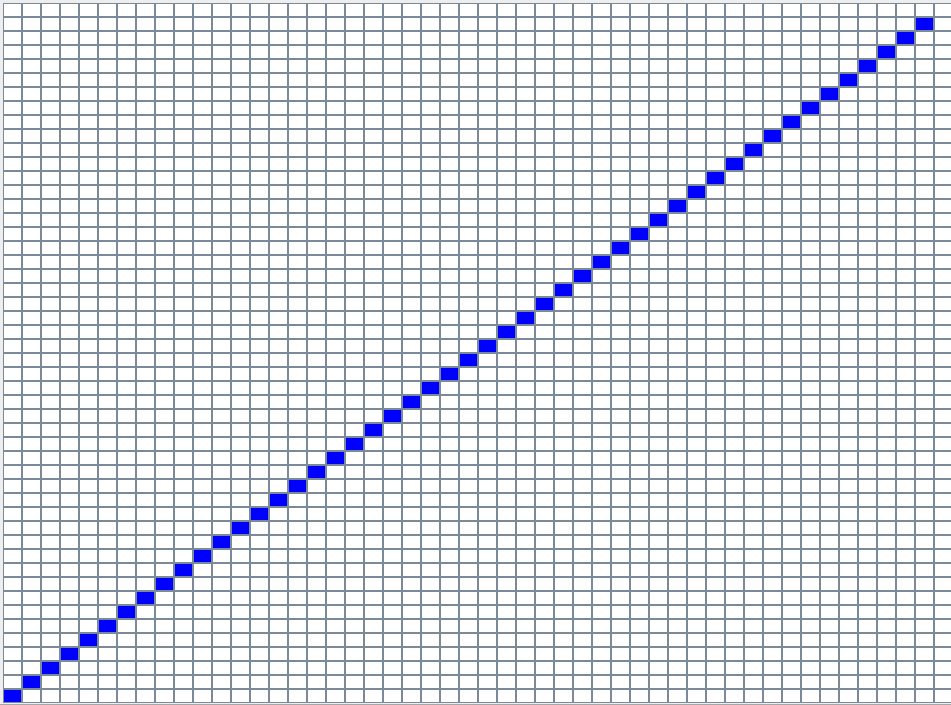
\includegraphics[scale=0.24]{ejemplo.png}
\caption{El tablero es blanco y está cuadriculado para la visibilidad.}
\end{center}
\end{figure}
\section*{Bonus (opcional)}
No solo muestre el resultado final de la ejecución del programa, si no que también los estados intermedios del tablero, es decir, muestre como la pluma ``colorea'' el tablero. Muestre animaciones que no terminan (note que esto no es posible en la versión de la tarea sin el bonus).
\section*{Referencias}
$[1]$ John Levine, \textit{Flex \& Bison : Text Processing Tools.} O'Reilly Media, Inc. 2009.\\ 
$[2]$ John Levine, Tony Mason, Doug Brown, \textit{Lex \& Yacc.} O'Reilly Media, Inc. 1992.
\end{document}
